\documentclass[12pt,letterpaper]{report}
\usepackage[margin=1in]{geometry}
\usepackage{titlesec}
\usepackage{amsmath}
\usepackage{amssymb}
\usepackage[colorlinks=true,urlcolor=black,linkcolor=black]{hyperref}
\usepackage{graphicx}
\usepackage{textcomp}
\usepackage{mathptmx}
\date{}
\usepackage{fullpage}
\usepackage{setspace}
\usepackage{hyperref}

\begin{document}
\begin{figure}
    \centering
    \begin{center}
          
\includegraphics[width=0.8\linewidth]{Images/img.jpg}
    \end{center}
\end{figure}
    \title{SOEN 6431 - Software Comprehension And Maintenance\\[1em]

   Deliverable 1 - Reengineering Opportunity\\ \textbf{DÉJÀ VU}}

\author{Submitted to : Dr. Pankaj Kamthan \\ \\
Summarized by:\\
A K M Saifun Nabi(40222168)\\
Dhruviben Jigeshkumar Modi(40166396)\\
Sumit Vasharambhai Monapara(40197174)\\
Harshal Jigeshkumar Modi (40195060)\\
\\\\
\centering
\href{https://github.com/mdhruvi/SOEN-6431-Deja-Vu}{Github Repository Link}\\
}
\maketitle
\pagebreak

\tableofcontents

\newpage
\addcontentsline{toc}{section}{1. Abstract}
\section*{1. Abstract}
\normalsize { Effective systems frequently undergo frequent updates, including improvements, to their source code. However, these changes could lead to a drop in quality, particularly in terms of efficiency and maintainability. It is significant to highlight that maintainability is a problem for software engineers but efficiency is a matter for users. At several levels, such as the software architecture, design, and implementation, the quality of the code might deteriorate. Reengineering strategies can be used to alleviate the deterioration in code quality. Refactoring is one such method that can be used with a variety of programming paradigms and languages.\\

From a list of four repositories recommended by our team members, we chose the candidate repository R for this work. Our investigation starts with a thorough examination of the "undesirables" present in the TeamScale-enabled repositories, such "undesirable" as inadequate code quality, a dearth of documentation, a complex code structure, and a lack of design patterns. We then focus on the candidate repository R because of particular justifications mentioned in the report. By selecting candidate R, we intend to start a reengineering process that addresses the noted "undesirables" and eventually improves the effectiveness and maintainability of the product.
}

\addcontentsline{toc}{section}{2. Introduction}
\section*{2. Introduction}
\normalsize {Software maintenance offers several advantages that contribute to the long-term success and effectiveness of software systems. Maintenance helps prevent the high expenses involved in creating brand-new software systems from beginning. It guarantees that software systems stay current and in line with changing consumer demands and technical improvements. It enables the detection and reduction of security threats and vulnerabilities. Higher user satisfaction results from well-maintained software systems. Software can be adapted to match user expectations and deliver the best user experience by fixing user-reported concerns and incorporating user feedback.\\

Reengineering in software maintenance is the process of reorganising or changing an existing software system in order to enhance its performance, quality, or other desirable qualities. It entails making significant adjustments to the software's architecture, methodology, or implementation without changing its functionality or user interface. Using TeamScale, we perform a preliminary analysis on four different repositories, identifying five separate flaws or "undesirables" for every repository. The quality of the repository's source code and documentation are then examined to determine whether a specific repository—designated candidate R—is appropriate for the reengineering process. \\

Following the successful selection of system R, we focus on further researching the "undesirables". We also want to implement the fixes for the issues found in selected system R by conducting Reengineering operationalization, it describes the actual application of the reengineering process in software development. in the following assignment.}

\newpage
\addcontentsline{toc}{section}{3. Project Deliberation}
\section*{3. Project Deliberation}
\addcontentsline{toc}{subsection}{3.1. Roles and Responsibility Matrix}
\subsubsection*{3.1. Roles and Responsibility Matrix}
\normalsize {Each team member was given the assignment of looking for a repository containing a software system in order to identify the potential system in accordance with the project specifications. We discussed the arguments against each scheme during a prearranged meeting. All systems were found to have drawbacks, which are described in the Repudiation justification for each system. The task of creating a paragraph outlining the justifications for rejecting every system but the selected one was then given to team members. To better prepare for the future deliverables, the team was segmented based on individual capabilities in documentation and coding.}

\begin{table}[h!]
\begin{tabular}{|l|l|l|l|l|l|}
\hline
\multicolumn{1}{|c|}{\begin{tabular}[c]{@{}c@{}}DEJA-VU\\ DELIVERABLE-1\end{tabular}} & {\begin{tabular}[c]{@{}c@{}}A K M Saifun Nabi\end{tabular}} & {\begin{tabular}[c]{@{}c@{}}Harshal Modi\end{tabular}} & {\begin{tabular}[c]{@{}c@{}} Dhruvi Modi\end{tabular}} & {\begin{tabular}[c]{@{}c@{}} Sumit Monapara\end{tabular}}\\ 
\hline
Research                                                               
& $\checkmark$                  & $\checkmark$                 & $\checkmark$                 & $\checkmark$                      \\ 
\hline
Brainstoming                                                                  & $\checkmark$                & $\checkmark$              &                  &                       \\ \hline
Collaborating                                                                &                 &                 & $\checkmark$               & $\checkmark$                   \\ \hline
Documentation                                                                 & $\checkmark$                & $\checkmark$               & $\checkmark$                  & $\checkmark$                        \\ \hline
\end{tabular}
\end{table}
\addcontentsline{toc}{subsection}{3.2. Factors for System Selection}
\subsection*{3.2. Factors for System Selection}
\normalsize{\textbf{Familiarity of Programming language :}\\
After evaluating the expertise of each team member, we determined that Java is the most suitable programming language for our project. Since all team members have significant experience using Java as their primary development language, any application that does not utilize Java will be given lower priority. That's why we give the first priority to java for our Project.}\\
\\
\normalsize{\textbf{Complex Programming Structure :}\\
We prioritize applications that are easy to set up since they require less time for project configuration. This allows us to allocate more hours towards analyzing the project and ensuring it meets the metrics of a potential system. we show complex structure in some projects in which we can not understand the flow of the code.}\\
\\
\normalsize{\textbf{Maintability :}\\
Even after deployment there is a possibility of bugs or updates in any existing feature of a software which makes it important to ensure that the software is maintained even after a successful deployment. A well maintained project also helps in reducing technical debt by code refactoring methods and also improves code quality.}\\
\pagebreak

\addcontentsline{toc}{section}{4. System Description}
\section*{4. System Description}
\addcontentsline{toc}{subsection}{4.1. Text Editor Application}
\subsection*{4.1. Text Editor Application - A K M Saifun Nabi } \\
\normalsize {\textbf{Project Description:}} \\
\normalsize {A Java-coded smart text editor/processor is a sophisticated software application that incorporates intelligent features commonly found in modern text interfaces. This text editor goes beyond basic functionality by offering advanced capabilities such as autocomplete, flagging misspelled words, and spelling auto-correction. It empowers users to produce error-free and polished text by offering real-time assistance and reducing the need for manual proofreading and correction.  It uses algorithms or language dictionaries to compare the input against a predefined set of correct words, providing visual cues to indicate potential errors. }\\
\\
\normalsize{\textbf{Source Code :}} 
\normalsize{\ https://github.com/salimt/Text-Editor-App/tree/master }\\
\\
\normalsize{\textbf{Programming Languages :}}
\normalsize{Java, CSS(Casceding Style Sheet), JUnit Testing.}\\
\\
\normalsize{\textbf{Repudiation Rationale : }}
\begin{itemize}
    \item \textbf{Lack of Modularity:} The code combines multiple concerns within the same class, violating the principle of separation of concerns. The controller class (for example: TextProController) contains UI controls, event handlers, initialization logic, and even business logic. This makes the code harder to understand, maintain, and test.
    \item \textbf{Tight Coupling and Lack of Dependency Injection: }The code directly creates instances of dependencies (for example: LaunchClass, AutoSpellingTextArea) within the controller class. This creates tight coupling and reduces flexibility. 
    \item \textbf{Non-Descriptive Naming:} Some variable names, such as li and adjustSpacing etc, are not descriptive and do not convey the purpose or intent of the variables. Using more meaningful and descriptive names would enhance the readability and maintainability of the code.
    \item \textbf{Lack of comments and documentation:} The code lacks sufficient comments and documentation to explain its purpose, algorithms, and assumptions which could impact maintainability in the long run.
    \item \textbf{Hardcoded Values:} There are several hardcoded values within the code, such as spacing values (for example: DEFAULTSPACING, SPACEDIV) and control thresholds (for example: RBOXTHRESHOLD, BUTTONWIDTH). Extracting these values into named constants with meaningful names would improve code readability and maintainability.
    \item \textbf{Testability:} The code does not explicitly show a testable design. Applying test-driven development (TDD) principles and writing automated tests would enhance the maintainability of the codebase.
\end{itemize}



\addcontentsline{toc}{subsection}{4.2. ATM Management System}
\subsection*{4.2. ATM Management System - Sumit Monapara} \\
\normalsize {\textbf{Project Description:}} \\
\normalsize {The ATM Management System is a Java project designed to simplify the management of customer accounts through an automated teller machine (ATM). It comprises classes such as Admin, AccountData, AfterLogin, and LoginForm, working together to ensure efficient account management and user-friendly interactions.The Admin class facilitates essential administrative tasks, including adding, deleting, and editing accounts, as well as saving account data. The AccountData class stores customer account information such as PIN codes, customer names, account types, account numbers, and starting balances.AfterLogin allows authenticated users to perform operations such as depositing funds, making withdrawals, checking balances, and conducting other account-related tasks. The LoginForm class provides a user-friendly interface for login authentication, validating credentials and granting access to the system upon successful login.This project streamlines account management, automates banking services, and enhances the overall user experience.}\\
\\
\normalsize{\textbf{Source Code :}} \\
\normalsize{\  https://github.com/zaahidali/ATM-Management-System.git }\\
\\
\normalsize{\textbf{Programming Languages :}}\\
\normalsize{Java Servlets(Java), Java Swing,  }\\
\\
\normalsize{\textbf{Repudiation Rationale : }}\\
\begin{itemize}
    \item \textbf{Lack of SCM integration:} The developer didn't utilize the feature of SCM to manage the versions of code, as the application is being developed. The code was directly uploaded to Github without integration locally at once when the application finally finished.
    \item \textbf{Lack of Maintenance:} The code is not properly maintained. There were only a few commits on the SCM back in 2020, and that too of updating the \textbf{README.md} file, not actual code is being committed. And then the latest commit is in 2023, of the same \textbf{README.md} file.
    \item \textbf{Security issue: } The application is of the ATM management system, which is considered a data-sensitive application, but here developer uses a text file to store sensitive data, which is vulnerable in terms of security, instead developer should have used secure database such as MySQL, MongoDB, etc. 
   
    \item \textbf{Testability:} The code does not contains test cases, on which we can perform Testing to identify the threats or bugs, that's why this application is not following TDD principles.
\end{itemize}
\\
\pagebreak



\addcontentsline{toc}{subsection}{4.3. Billing-System}
\subsection*{4.3. Billing-System - Dhruvi Modi } \\
\normalsize {\textbf{Project Description:}} \\
\normalsize {The Java-coded GUI-based Complete Store Billing System is a comprehensive software project designed to streamline the billing process in a store environment. This application is developed using Java Swing and Java AWT, two popular Java libraries for creating graphical user interfaces. With this system, store owners or cashiers can easily generate invoices for each sale made in the store. The graphical user interface provides a visually appealing and interactive platform for managing the billing operations. Using Java Swing and Java AWT, the project offers a wide range of graphical components, including buttons, text fields, drop-down menus, and tables, to facilitate user interactions. The GUI elements are organized in a user-friendly manner, allowing users to navigate through the application effortlessly. }\\
\\
\normalsize{\textbf{Source Code :}} \\
\normalsize{\ https://github.com/AmbalviUsman/Billing-System/blob/master/src/AdminPanel.java}\\
\\
\normalsize{\textbf{Programming Languages :}}\\
\normalsize{Java Swing, Java AWT.}\\
\\
\normalsize{\textbf{Repudiation Rationale : }}\\
\begin{itemize}
    \item \textbf{Testability: }The codebase would benefit from a design that explicitly supports testability. By applying principles of test-driven development (TDD) and writing automated tests, the maintainability of the code can be improved. So adding test cases with the use of Junit will be improved the quality of code.
    \item \textbf{Lack of Maintenance: }The codebase lacks proper maintenance as evidenced by infrequent commits on the source code management (SCM) system. The README.md file is not also organized properly. There is not proper information about the proeject in README.md file and there were very few commits in it.
    \item \textbf{Lack of Issue Resolution in GitHub Repository: } There are four issues raised in this project but that issues are not solved by the owner. He does not provided the proper dataset and there is some naming error in the variables of the code nut it can not be solevd.
    \item \textbf{Lack of documentation and comments: } Insufficient comments and documentation are evident in the code, making it difficult to understand the purpose, algorithms, and underlying assumptions. This lack of explanatory information could have a negative impact on the long-term maintainability of the codebase.
\end{itemize}
\\
\normalsize{\textbf{According to section (6), the aforementioned project is chosen as the system R based on a variety of criteria. }}\\
    
\\

\addcontentsline{toc}{subsection}{4.4. Hospital Management System}
\subsection*{4.4. Hospital Management System - Harshal Modi } \\
\normalsize {\textbf{Project Description:}} \\
\normalsize {The Hospital Management System is a Java-based project that utilizes the Java AWT (Abstract Window Toolkit) and GUI (Graphical User Interface) components to create a comprehensive system for managing hospital operations. This project aims to streamline and automate various administrative tasks within a hospital setting. It provides a user-friendly interface in the form of interactive forms, allowing hospital staff to efficiently manage patient records, appointments, and other crucial information. The Hospital Management System allows authorized personnel, such as doctors, nurses, and administrative staff, to access and update patient records, view appointment schedules, and manage hospital resources effectively. The system incorporates features like data validation and error handling to ensure the accuracy and integrity of the information stored.}\\
\\
\normalsize{\textbf{Source Code :}} \\
\normalsize{https://github.com/Prabashi/HospitalManagementSystem/tree/master/src/com/gui}\\
\\
\normalsize{\textbf{Programming Languages :}}\\
\normalsize{Java Swing, AWT, SQL}\\
\\
\normalsize{\textbf{Repudiation Rationale : }}\\
\begin{itemize}
    \item \textbf{No Documentation:} This repository doesn't contain \textbf{README} file, which is the primary resource for documentation for the GitHub repository, which guides the external user on how to install, build, run, and use the application. Without \textbf{README} file we can not understand the flow of the code and we do not get the whole idea about the functionality of each class and each methods. 
    \item \textbf{Testability:} The code lacks explicit definition of test cases to thoroughly test and cover the code. This absence hinders the ability to perform code coverage analysis and unit testing, which are essential components of test-driven development (TDD) for application code.
    \item \textbf{No Maintainability :} The code on the GitHub repository has not received any maintenance or updates since the last commit in 2018. The absence of ongoing maintenance raises concerns about the code's current state, bug fixes, and compatibility with newer technologies or dependencies. It is important to regularly maintain code to ensure its stability, security, and alignment with evolving best practices. The lack of recent maintenance in the code structure suggests the need for attention and potential updates to address any issues and maintain the codebase effectively.
    \item \textbf{Complex Code Structure:} When dealing with a complex code structure where lines of code become excessively long, it can significantly impact readability, maintainability, and the overall quality of the codebase. The codebase has in total greater than 2K Line of code which is very complicate to read.
    
\end{itemize}
\\
\pagebreak


\newpage
\addcontentsline{toc}{section}{5. Selected System Description}
\section*{5. Selected System Description}
\normalsize \textbf{Billing System}

\addcontentsline{toc}{subsection}{5.1. Purpose}
\subsubsection*{5.1. Purpose}
\normalsize {Each team member was given the assignment of looking for a repository containing a software system in order to identify the potential system in accordance with the project specifications. We discussed the arguments against each scheme during a prearranged meeting. All systems were found to have drawbacks, which are described in the Repudiation justification for each system. The task of creating a paragraph outlining the justifications for rejecting every system but the selected one was then given to team members. To better prepare for future deliverables, the team was segmented based on individual capabilities in documentation and coding.}
\\
\\
\begin{figure}[ht]
    \centering
    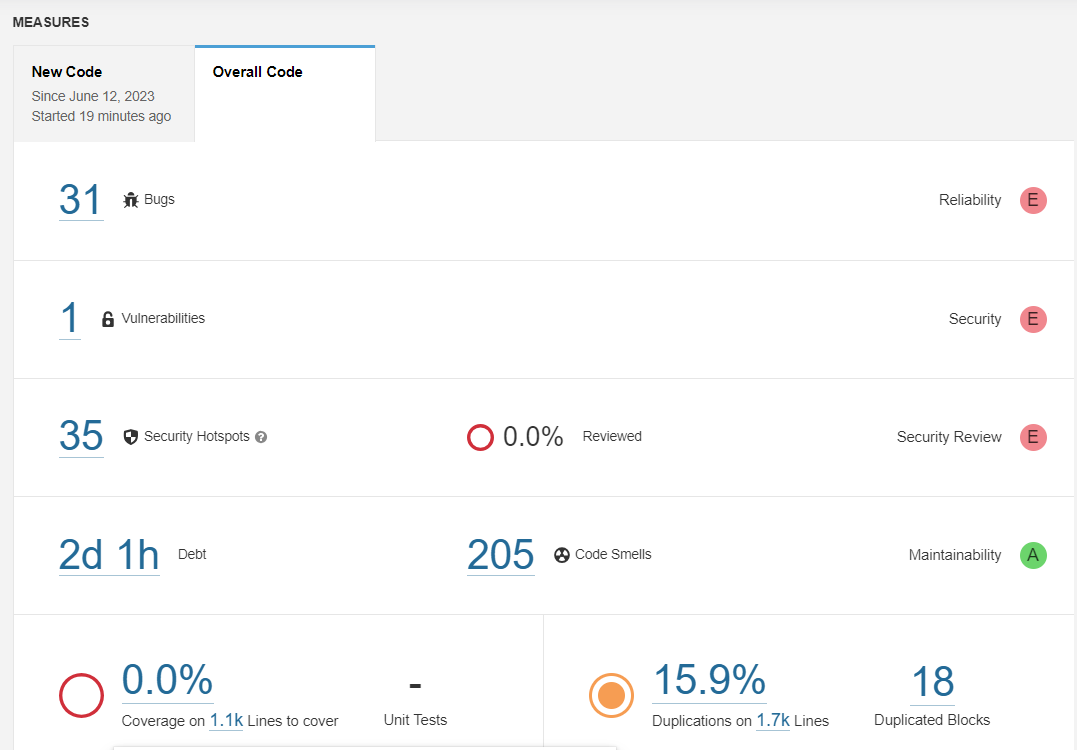
\includegraphics[width=0.8\linewidth]{Images/sonar_report.png}\
    \caption{SonarQube Analysis of the selected application (Billing System)}
    \label{fig:enter-label}
\end{figure}

\normalsize {As we can see in the above image, the selected application contains various bugs, several Vulnerabilities issues, and not following standard language rules and syntax, hence not passing the Quality gate, and in addition to that, there were no Unit test cases defined, through which we can identify the code coverage, hence the code coverage shows 0.0\% in the sonar analysis report. So we will try to resolve this issue in the next deliverable}

\pagebreak
\addcontentsline{toc}{subsection}{5.2. Programming Language}
\subsubsection*{5.2. Programming Language}
\normalsize {There are various advantages to using Java as the programming language to create a CRUD (Create, Read, Update, Delete) application for a billing system.}

\begin{itemize}
    \item \textbf{Platform Independence: }Java is renowned for its "write once, run anywhere" approach, according to which Java programmes can be launched on any platform that has a Java Virtual Machine (JVM). This makes it possible to implement the billing system without having to make significant changes on several operating systems, including Windows, macOS, and Linux.

    \item \textbf{Rich GUI Capabilities: }The graphical user interface (GUI) modules and components offered by Java Swing enable programmers to design interactive and aesthetically pleasing interfaces for the billing system. The user experience can be improved by using Java Swing to provide an interface with elements like buttons, menus, tables, and forms.

    \item \textbf{Database Connectivity: }JDBC (Java Database Connectivity) enables interaction with databases and seamless database integration, which enables the billing system to store and retrieve data quickly. The programme can quickly connect to many database management systems, run queries, and carry out CRUD tasks using JDBC. 

    \item \textbf{Object-Oriented Programming (OOP): } The OOP paradigm, which Java adheres to, encourages modular and reusable code. This makes it simpler to design and implement the many Billing System components as distinct and cohesive entities, such as the customer management, product inventory, and billing modules. 

    \item \textbf{Resources and Community Support: }Since Java has a sizable and vibrant developer community, there are a tonne of online resources, tutorials, and forums accessible for direction and support during the development process. With the help of the community, developers can be sure that they can overcome any obstacles they may face while they create the Billing System.


\end{itemize}


\newpage
\addcontentsline{toc}{section}{6. Selected System Rationale}
\section*{6. Selected System Rationale}

\addcontentsline{toc}{subsection}{6.1. Technical Reasons}
\subsubsection*{6.1. Technical Reasons}
Each team given to team members. To better prepare for the future deliverables, the team was segmented based on individual capabilities in documentation and coding.
\begin{itemize}
    \item \textbf{Language Familiarity:} All our Team members are familier with java language. Since all team members are already familiar with Java, choosing a Java project ensures that everyone can contribute effectively right from the start. It eliminates the need for additional time and effort to learn a new programming language, allowing the team to focus on the project's technical aspects and deliverables.
    \item \textbf{Scalability and Performance:} Java's scalability and performance make it a suitable choice for a billing system. Java applications can handle large amounts of data and concurrent users efficiently. With its support for multithreading and high-performance frameworks like Spring Boot, Java can handle the computational demands of real-time billing calculations and processing without sacrificing performance.
    \item \textbf{Coding Design Pattern:} In our Selected Project Billing System He follows proper coding structure MVC(Model View Controller) in which he designs different java classes like login java file, sales java file, product java file etc. He also maintains the naming conventions for each java classes. He also uses java swing class properly and added images folder separately. 
    \item \textbf{Exception Handling:} Java has a robust exception handling mechanism, which is crucial for a billing system. The system may encounter various exceptional scenarios, such as invalid input data, network issues, or database errors. Java's exception handling allows you to gracefully handle these exceptions, log relevant information, and take appropriate actions, ensuring the system's reliability and stability. So He follows proper Exception handling in his project for invalid data or empty dataset.
    \item \textbf{Database Integration:} Billing systems typically require seamless integration with databases to store and retrieve customer data, invoices, payment information, etc. Java offers a variety of libraries and frameworks for database integration, including JDBC (Java Database Connectivity) and popular ORM (Object-Relational Mapping) frameworks like Hibernate. These tools simplify database interactions and provide efficient data access, reducing development effort and ensuring proper data management in the billing system. He uses proper JDBC connection queries for dataset integraion.  
\end{itemize}

\newpage
\addcontentsline{toc}{subsection}{6.2. Non-technical Reasons}
\subsubsection*{6.2. Non-technical Reasons}
\normalsize {Below are the non-technical reasons which motivate us  beyond technical aspects to work on this codebase.}

\begin{itemize}
    \item \textbf{User experience: }Improving the user interface and overall user experience of the billing process is a motivation to choose this project. Enhancing the design, layout, and usability aspects can make it easier and more intuitive for users to use the software.
    \item \textbf{Efficiency and automation:} Working on the code can involve automating certain aspects of the billing process, such as retrieving customer information from a database, calculating taxes or discounts, or generating invoice numbers automatically. Improving efficiency and reducing manual efforts are other reasons to work on this project.
    \item \textbf{Collaboration and teamwork:} Collaborating on the code is an opportunity to foster teamwork and improve communication among our team members. Working together to enhance the code can lead to shared understanding, knowledge transfer, and improved collaboration among us.
    \item \textbf{Scalability and future growth:} There is a possibility an increasing number of customers needs to be handled, and working on the code involves optimizing performance and scalability aspects.
    \item     \textbf{Code quality and maintainability:} Working on the code is also influenced by a desire to improve its overall quality and maintainability. Refactoring the code to follow best practices, reducing code duplication, and improving its structure will make it easier to maintain, understand, and enhance in the future.
\end{itemize}

\clearpage
\addcontentsline{toc}{section}{7. References}
\section*{7. References}

\href{https://www.sealights.io/software-quality/software-maintainability-what-it-means-to-build-maintainable-software/}{1. What it Means to Build Maintainable Software. [Online].\\
 \href{https://ecomputernotes.com/software-engineering/coding-documentation}{2. Coding Documentation in Software Engineering [Online]. }\\
 \href{https://www.parasoft.com/blog/how-to-write-test-cases-for-software-examples-tutorial/}{3. William McMullin, How to Write Test Cases for Software, May 27, 2021. [Online].}.\\

\href{https://www.sealights.io/software-quality/software-maintainability-what-it-means-to-build-maintainable-software}{1. "What it Means to Build Maintainable Software," [Online].}\\
 \href{https://ecomputernotes.com/software-engineering/coding-documentation}{2. "Coding Documentation in Software Engineering"[Online]. }\\
 \href{https://www.parasoft.com/blog/how-to-write-test-cases-for-software-examples-tutorial}{3. William McMullin, How to Write Test Cases for Software, May 27, 2021. [Online]}.\\
 \href{https://www.netsolutions.com/insights/software-design-pattern/}{4.  Lalit Singla, Design Patterns, January 05, 2022. [Online].}\\
 \href{https://rewind.com/blog/best-practices-for-using-github-issues/}{5. Jura Gorohovsky, Best practices for using GitHub Issues, April 13, 2023. [Online].}\\
 \href{https://www.altexsoft.com/blog/business/technical-documentation-in-software-development-types-best-practices-and-tools/}{6. Technical Documentation in Software Development [Online].}\\
 \href{https://docs.sonarqube.org/latest/}{7. SonarQube (Tool used to analyze the application code)}\\
 \href{https://docs.sonarqube.org/latest/analyzing-source-code/scanners/sonarscanner/}{8. CLI tools used by sonar, SonarScanner}
 
\end{document}